\documentclass{article}
\usepackage{parskip}
\usepackage{amsmath}
% use UTF8 encoding
\usepackage[utf8]{inputenc}
% use KoTeX package for Korean
\usepackage{kotex}
\usepackage{hyperref}
\usepackage{enumitem}
\usepackage{matlab-prettifier}
\usepackage{geometry}
\usepackage{graphicx}
\usepackage{hyperref}
\hypersetup{
    colorlinks=true,
    linkcolor=blue,
    filecolor=magenta,      
    urlcolor=cyan,
    pdftitle={Overleaf Example},
    pdfpagemode=FullScreen,
}

\geometry{
    a4paper,
    left=30mm,
    right=30mm,
    top=30mm,
    bottom=40mm
 }

\hypersetup{
    colorlinks=true,   
    urlcolor=red,
}

\begin{document}

\title{Assignment 3}
\author{20180282 Jimin Park}
\maketitle

\begin{enumerate}
    \item First, put
    \begin{align*}
        x_0 = -1, x_1 = 1, x_2 = 2,
        \\
        y_0 = 2, y_1 = 0, y_2 = 2,
        \\
        y_0^\prime = 1, y_1^\prime = 1, y_2^\prime = 3.
    \end{align*}
    Also, put
    \begin{align*}
        z_0 = z_1 = -1, z_2 = z_3 = 1, z_4 = z_5 = 2.
    \end{align*}
    Now, we can put the Hermite interpolating polynomial $H_5(x)$ by
    \begin{align}
        H_5(x) = a_0 + a_1(x-z_0) + \cdots + a_5(x-z_0)\cdots(x-z_5).
    \end{align}
    Then we can make divided difference table as below:
    \begin{align*}
        \begin{array}{|l|c|c|c|c|c|c|}
            \hline
            z_0 & f[z_0] &                              &&&&
            \\
            \hline
            z_1 & f[z_1] & f[z_0, z_1] = f^\prime(z_1)  &&&&
            \\
            \hline
            z_2 & f[z_2] & f[z_1, z_2]                  & f[z_0, z_1, z_2] &&&
            \\
            \hline
            z_3 & f[z_3] & f[z_2, z_3] = f^\prime(z_3)  & f[z_1, z_2, z_3] & f[z_0, \cdots, z_3] &&
            \\
            \hline
            z_4 & f[z_4] & f[z_3, z_4]                  & f[z_2, z_3, z_4] & f[z_1, \cdots, z_4] & f[z_0, \cdots, z_4] &
            \\
            \hline
            z_5 & f[z_5] & f[z_4, z_5] = f^\prime(z_5)  & f[z_3, z_4, z_5] & f[z_2, \cdots, z_5] & f[z_1, \cdots, z_5] & f[z_0, \cdots, z_5]
            \\
            \hline
        \end{array}
    \end{align*}
    Now, let's compute the entires of the table. Then we get the below table:
    \begin{align}
        \begin{array}{|l|c|c|c|c|c|c|}
            \hline
            -1 & 2 &    &&&&
            \\
            \hline
            -1 & 2 & 1  &&&&
            \\
            \hline
            1 & 0 & -1  & -1    &&&
            \\
            \hline
            1 & 0 & 1   & 1     & 1 &&
            \\
            \hline
            2 & 2 & 2   & 1     & 0 & -\frac{1}{3}  &
            \\
            \hline
            2 & 2 & 3   & 1     & 0 & 0             & \frac{1}{9}
            \\
            \hline
        \end{array}
    \end{align}
    Note that
    \begin{align*}
         a_n = f[z_0, \cdots, z_n].
    \end{align*}
    Hence, we get
    \begin{align}
        \begin{split}
            H_5(x) = & 2 + (x+1) - (x+1)^2 + (x+1)^2(x-1)
            \\ & - \frac{1}{3}(x+1)^2(x-1)^2 + \frac{1}{9}(x+1)^2(x-1)^2(x-2)
        \end{split}
    \end{align}
    \item Below is my code. \begin{lstlisting}[frame=single, numbers=left, style=Matlab-editor]
% Set our function
syms x
f(x) = (x^2 + 1)^(-1);

% Set inputs and outputs
inputs = linspace(-5, 5, 21);
a = f(inputs);
b = zeros(1, 20);
c = zeros(1, 21); % For Step 5&6. c(21) is not output.
d = zeros(1, 20);

% Step 1
h = inputs(2) - inputs(1);

% Step 2
alpha = zeros(1, 20);
for i = 2:20
    alpha(i) = 3/h*(a(i+1)-a(i)) - 3/h*(a(i)-a(i-1));
end

% Step 3
l = zeros(1, 21);
l(1) = 1;
mu = zeros(1, 21);
z = zeros(1, 21);

% Step 4
for i = 2:20
    l(i) = 4*h - h*mu(i-1);
    mu(i) = h/l(i);
    z(i) = (alpha(i) - h*z(i-1)) / l(i);
end

% Step 5
l(21) = 1;
z(21) = 0; % actually z = zeros(1, 21) already implies this
c(21) = 0; % actually c = zeros(1, 21) already implies this

% Step 6
for j = 20:-1:1
    c(j) = z(j) - mu(j)*c(j+1);
    b(j) = (a(j+1) - a(j)) / h - h * (c(j+1) + 2*c(j)) / 3;
    d(j) = (c(j+1) - c(j)) / (3*h);
end

% Step 7: Plotting
X = linspace(-5, 5, 51)
Y = zeros(1, 51);

S(x) = a(1) + b(1)*(x-inputs(1)) + c(1)*(x-inputs(1))^2 + d(1)*(x-inputs(1))^3;
j = 1;
for i = 1:51
    if inputs(j+1) < X(i)
        j = j + 1;
        S(x) = a(j) + b(j)*(x-inputs(j)) + c(j)*(x-inputs(j))^2 + d(j)*(x-inputs(j))^3;
    end
    Y(i) = S(X(i)) - f(X(i));
end
disp(Y);
plot(X, Y);        
    \end{lstlisting} Then we get the values of $S(x)-f(x)$ at 51 equally spaced points and the corresponding graph (Fig. 1). \begin{lstlisting}[frame=single, numbers=left, style=Matlab-editor]
0    0.0001    0.0000   -0.0000   -0.0000    0.0000    0.0000    0.0000   -0.0000   -0.0000   -0.0000   -0.0000    0.0000   -0.0000   -0.0001    0.0000    0.0001    0.0001   -0.0003   -0.0009   -0.0000    0.0029    0.0019   -0.0015   -0.0021    0.0000   -0.0021   -0.0015    0.0019    0.0029   -0.0000   -0.0009   -0.0003    0.0001    0.0001   -0.0000   -0.0001   -0.0000    0.0000   -0.0000    0.0000   -0.0000   -0.0000    0.0000    0.0000    0.0000   -0.0000   -0.0000    0.0000    0.0001   -0.0000
    \end{lstlisting} \begin{figure}[h] %%% t: top, b: bottom, h: here
        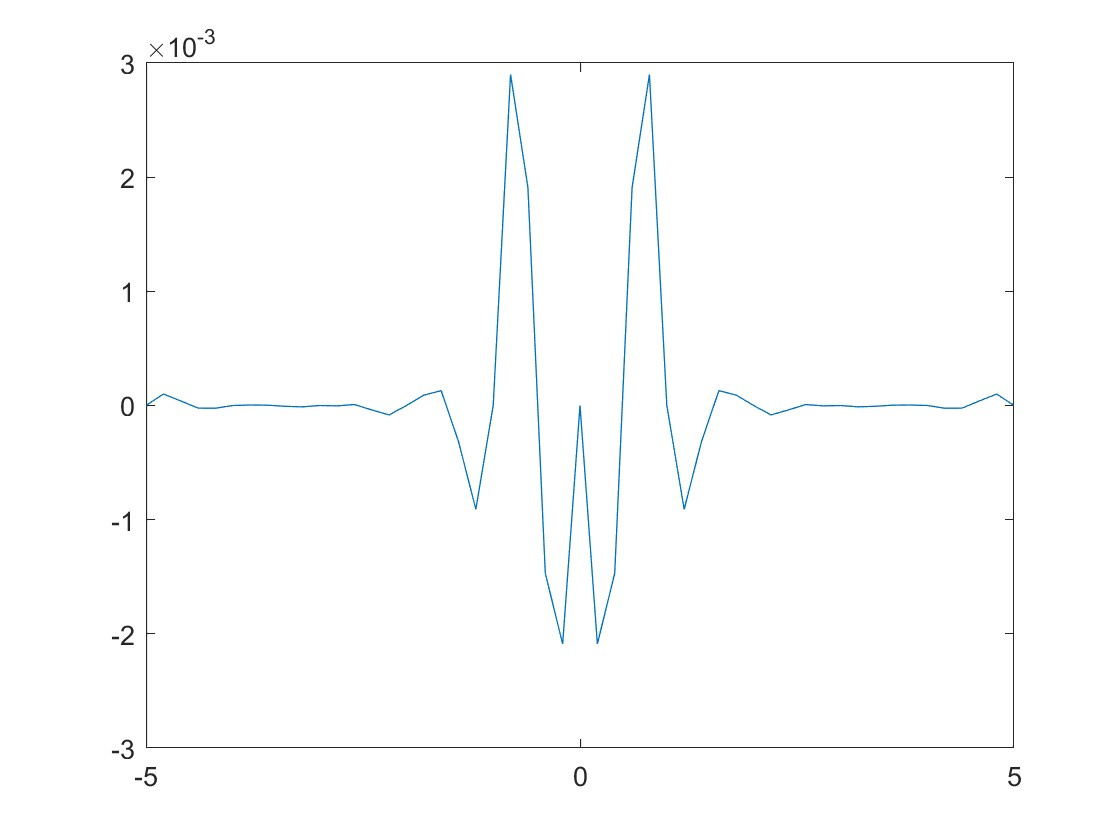
\includegraphics[width=0.9\textwidth]{assignment_3_2_fig.jpg}
        \centering
        \caption{Plotting of $S(x)-f(x)$}
    \end{figure} Now, compare this problem with the Problem 4 of Assignment 2. In the Problem 4 of Assignment 2, we used Newton interpolating polynomial $P$ interpolating a function $f$. Since the degree of such polynomial is big, 20, it may oscillates a lot. Actually, we saw that $P(x)-f(x)$ is far from zero near $x=-5, 5$. But for the cubic spline polynomial, since this is a piecewise polynomial with relatively low degree, 3, $S(x)-f(x)$ is near zero in the entire interval $[-5, 5]$. Of course, the value of $P(x)-f(x)$ and $S(x)-f(x)$ are both zero at node points, $x=x_j,\ j=0,1,2,\cdots,20$.

    \item \begin{enumerate}[wide=10pt]
        \item By the two-point forward formula, we get \begin{align*}
            f^\prime(x) = \frac{1}{h}[f(x+h)-f(x)]-\frac{h}{2}f^{\prime\prime}(\xi)
        \end{align*} where $\xi$ is between $x$ and $x+h$. Let $\tilde{\cdot}$ represent the floating number approximation (computed by computer) and $e$ is corresponding round-off error. Then \begin{align*}
            f^\prime(x) = \frac{1}{h}[\tilde f(x+h)-\tilde f(x)] + \frac{1}{h}[e(x+h)-e(x)] -\frac{h}{2}f^{\prime\prime}(\xi).
        \end{align*} Now, assume that the round-off $e(x)$ and $e(x+h)$ are bounded by some number $\epsilon>0$ and the second derivative of $f$ is bounded by a number $M>0$, then \begin{align}
            \left | f^\prime(x) - \frac{1}{h}[\tilde f(x+h)-\tilde f(x)] \right |
            \le \frac{2\epsilon}{h} + \frac{hM}{2}.
        \end{align} Here, by the arithmetic mean-geometric mean inequality, we can get the minimum bound for the bound of the error \begin{align*}
            \frac{2\epsilon}{h} + \frac{hM}{2} \ge 2\sqrt{\epsilon M},
        \end{align*} and the equality holds when $\frac{2\epsilon}{h}=\frac{hM}{2}$, i.e., when $h=2\sqrt{\epsilon /M}$. We can get $\epsilon$ by typing 'eps' in the MATLAB and can simply put $M=1$ since $f^{\prime\prime}(x)=-\cos x$. Note that eps value is $2.220446049250313\times 10^{-16}$. Hence we get the minimum bound for the error when \begin{align} \label{eqn:h_val_1}
            h = 2\sqrt{\frac{\epsilon}{M}} = 2\sqrt{2.220446049250313\times 10^{-16}} \approx 3\times 10^{-8}.
        \end{align}
        
        Until now, we estimate the minimum error using the theorem with what we learned in the class. But actually, round-off error eps is just the upper bound for the round-off error, but not the least upper bound. So the value of $h$ that estimates derivative could be smaller than (\ref{eqn:h_val_1}). With this notice, I estimate the derivative using smaller $h$ as well as (\ref{eqn:h_val_1}). Below is my code for estimating derivative: \begin{lstlisting}[frame=single, numbers=left, style=Matlab-editor]
format long;

syms x h;
f(x) = cos(x);
N1(x, h) = (f(x+h) - f(x))/h;

h0 = 3 * 10^(-8);
a = -sin(0.25);
b = double(N1(0.25,h0));
e = rel_error(a, b);

fprintf("f'(0.25) is: %.15f\n", a);
fprintf("estimated value is: %.15f\n", b);
fprintf("relative error is: %.15e\n\n", e);

h0 = 10^(-17);
b = double(N1(0.25,h0));
e = rel_error(a, b);

fprintf("f'(0.25) is: %.15f\n", a);
fprintf("re-estimated value is: %.15f\n", b);
fprintf("relative error is: %.15e\n", e);

function e = rel_error(real_val, estimated_val)
    e = abs((real_val - estimated_val) / estimated_val);
end
        \end{lstlisting} And the below is the result: \begin{lstlisting}[frame=single, numbers=left, style=Matlab-editor]
f'(0.25) is: -0.247403959254523
estimated value is: -0.247403973788209
relative error is: 5.874475684322718e-08

f'(0.25) is: -0.247403959254523
re-estimated value is: -0.247403959254523
relative error is: 0.000000000000000e+00
        \end{lstlisting}
        \item Put \begin{align}
            N_1(h) := \frac{1}{h}[f(x+h)-f(x)].
        \end{align} Using Taylor series, we get \begin{align} \label{eqn:h1}
            f^\prime(x) = N_1(h) -\frac{f^{\prime\prime}(x)}{2}h - \frac{f^{(3)}(x)}{6}h^2 - \frac{f^{(4)}(x)}{24}h^3 - \cdots.
        \end{align} Taking $h/2$, we get \begin{align*}
            f^\prime(x) = N_1 \left (\frac{h}{2} \right ) -\frac{f^{\prime\prime}(x)}{2}\frac{h}{2} - \frac{f^{(3)}(x)}{6}\frac{h^2}{4} - \frac{f^{(4)}(x)}{24}\frac{h^3}{8} - \cdots.
        \end{align*} Multiplying it by 2 and subtracting (\ref{eqn:h1}), we get \begin{align*}
            f^\prime(x) = 2N_1 \left (\frac{h}{2} \right ) - N_1(h) + \frac{f^{(3)}(x)}{12}h^2 + \frac{3f^{(4)}(x)}{96}h^3 + \cdots.
        \end{align*} Then by putting \begin{align}
            N_2(h) := 2N_1 \left (\frac{h}{2} \right ) - N_1(h),
        \end{align} we can rewrite the equation as below: \begin{align} \label{eqn:h2}
            f^\prime(x) = N_2(h) + \frac{f^{(3)}(x)}{12}h^2 + \frac{3f^{(4)}(x)}{96}h^3 + \cdots.
        \end{align}
        
        Again, taking $h/2$ on (\ref{eqn:h2}), we get  \begin{align*}
            f^\prime(x) = N_2 \left (\frac{h}{2} \right ) + \frac{f^{(3)}(x)}{12}\frac{h^2}{4} + \frac{3f^{(4)}(x)}{96}\frac{h^3}{8} + \cdots.
        \end{align*} Multiplying it by 4 and subtracting (\ref{eqn:h2}), we get \begin{align*}
            3f^\prime(x) = 4N_2 \left (\frac{h}{2} \right ) - N_2(h) - \frac{3f^{(4)}(x)}{96}\frac{h^3}{2} - \cdots.
        \end{align*} Then by putting \begin{align}
            N_3(h) := \frac{1}{3} \left ( 4N_2 \left (\frac{h}{2} \right ) - N_2(h) \right ),
        \end{align} we can rewrite the equation as below: \begin{align} \label{eqn:h3}
            f^\prime(x) = N_3(h) - \frac{f^{(4)}(x)}{192}h^3 - \cdots.
        \end{align}

        Let's see $N_3(h)$ in detail. First, \begin{align*}
            N_2(h) & = 2\frac{2}{h}\left [f\left ( x + \frac{h}{2} \right ) - f(x) \right ] - \frac{1}{h}[f(x+h)-f(x)]
            \\ & = \frac{1}{h} \left [ -3f(x) + 4f\left (x + \frac{h}{2} \right ) - f(x+h) \right ].
        \end{align*} Therefore, \begin{align*}
            N_3(h) & = \frac{1}{3} \left( 4\frac{2}{h} \left[ -3f(x) + 4f \left(x+\frac{h}{4} \right) - f \left( x+\frac{h}{2} \right) \right] \right.
            \\ & \quad \quad \quad \left. - \frac{1}{h} \left[ -3f(x) + 4f\left(x + \frac{h}{2} \right) - f(x+h) \right] \right)
            \\ & = \frac{1}{3} \left(\frac{1}{h} \left[-21f(x)+32f\left(x+\frac{h}{4}\right)-12f\left(x+\frac{h}{2}\right)+f(x+h)\right] \right),
        \end{align*} i.e., \begin{align}
            N_3(h) = \frac{1}{3h}\left[-21f(x)+32f\left(x+\frac{h}{4}\right)-12f\left(x+\frac{h}{2}\right)+f(x+h)\right].
        \end{align}

        For the error bound, we can apply similar method of (a). We may write \begin{align*}
            f^\prime(x) = N_3(h) - \frac{h^3}{192}f^{(4)}(\xi),
        \end{align*} where $\xi$ is between $x$ and $x+h$. Then we get \begin{align}
            \begin{split}
                & \left| f^\prime(x) - \frac{1}{3h}\left[-21\tilde f(x)+32\tilde f\left(x+\frac{h}{4}\right)-12\tilde f\left(x+\frac{h}{2}\right)+\tilde f(x+h)\right] \right|
                \\ & \le \frac{22\epsilon}{h} + \frac{Mh^3}{192},
            \end{split}
        \end{align} where $\epsilon>0$ is the bound of the round-off error and $M>0$ is the bound of $f^{(4)}$. We can get $\epsilon$ by typing 'eps' in the MATLAB and can simply put $M=1$ since $f^{(4)}(x)=\cos x$. By calculating $h$ where the derivative of $\frac{22\epsilon}{h} + \frac{Mh^3}{192}$ is zero, we can know that this bound is minimum when \begin{align} \label{eqn:h_val_3}
            h = \left(1408\frac{\epsilon}{M}\right)^{1/4} = \left(1408\times 2.220446049250313\times 10^{-16}\right)^{1/4}
            \approx 7.5 \times 10^{-4}.
        \end{align}

        With the same reasoning in (a), I estimate the derivative using smaller $h$ as well as (\ref{eqn:h_val_3}). Below is my code for estimating derivative: \begin{lstlisting}[frame=single, numbers=left, style=Matlab-editor]
format long;

syms x h;
f(x) = cos(x);
N3(x, h) = 1 / (3 * h) * (-21*f(x) + 32*f(x+h/4) - 12*f(x+h/2) + f(x+h));

h0 = 7.5 * 10^(-4);
a = -sin(0.25);
b = double(N3(0.25,h0));
e = rel_error(a, b);

fprintf("f'(0.25) is: %.15f\n", a);
fprintf("estimated value is: %.15f\n", b);
fprintf("relative error is: %.15e\n\n", e);

h0 = 10^(-5);
b = double(N3(0.25,h0));
e = rel_error(a, b);

fprintf("f'(0.25) is: %.15f\n", a);
fprintf("re-estimated value is: %.15f\n", b);
fprintf("relative error is: %.15e\n", e);

function e = rel_error(real_val, estimated_val)
    e = abs((real_val - estimated_val) / estimated_val);
end
        \end{lstlisting} And the below is the result: \begin{lstlisting}[frame=single, numbers=left, style=Matlab-editor]
f'(0.25) is: -0.247403959254523
estimated value is: -0.247403959252394
relative error is: 8.604651682115397e-12

f'(0.25) is: -0.247403959254523
re-estimated value is: -0.247403959254523
relative error is: 0.000000000000000e+00
        \end{lstlisting}
    \end{enumerate}
    \item Let's consider a function $f\in C^4[x_0, x_3]$ and the Lagrange interpolating function $P_3(x)$ interpolating $f(x)$ at four points: $x_0, x_1, x_2, x_3$. Here, we assume that these points are equally spaced with distance $h$, i.e., $h = x_i-x_{i-1}$. By the theorem for the Lagrange interpolation function, for any $x \in [x_0, x_3]$ we can choose $\xi(x) \in [x_0, x_3]$ satisfying \begin{align}
        f(x) = P_3(x) + \frac{f^{(4)}(\xi(x))}{4!}(x-x_0)(x-x_1)(x-x_2)(x-x_3).
    \end{align}
    Now let's see $P_3(x)$ in detail. Let \begin{align*}
        P_3(x) = \sum_{i=0}^{3} a_i(x-x^*)^i,
    \end{align*} where $x^* = (x_0+x_3)/2$. Then by plugging in $x=x_k,\ k=0,1,2,3$, we get \begin{align*}
        f(x_0) = P_3(x_0) = a_0 - \frac{3}{2}ha_1 + \frac{9}{4}h^2a_2 - \frac{27}{8}h^3a_3,
        \\
        f(x_1) = P_3(x_1) = a_0 - \frac{1}{2}ha_1 + \frac{1}{4}h^2a_2 - \frac{1}{8}h^3a_3,
        \\
        f(x_2) = P_3(x_2) = a_0 + \frac{1}{2}ha_1 + \frac{1}{4}h^2a_2 + \frac{1}{8}h^3a_3,
        \\
        f(x_3) = P_3(x_3) = a_0 + \frac{3}{2}ha_1 + \frac{9}{4}h^2a_2 + \frac{27}{8}h^3a_3.
    \end{align*} Here, \begin{align*}
        f(x_0)+f(x_3) = 2a_0 + \frac{9}{2}h^2a_2,
        \\
        f(x_1)+f(x_2) = 2a_0 + \frac{1}{2}h^2a_2.
    \end{align*} Hence, we get \begin{align*}
        a_0 = \frac{1}{16}[-f(x_0)+9f(x_1)+9f(x_2)-f(x_3)],
        \\
        a_2 = \frac{1}{4h^2}[f(x_0)-f(x_1)-f(x_2)+f(x_3)].
    \end{align*} By integrating $P_3$ on $[x_0, x_3]$, we get \begin{align}
        \begin{split}
            \int_{x_0}^{x_3}P_3(x) dx
            & = \sum_{i=0}^{3}a_i \int_{x_0}^{x_3}(x-x^*)^i
            \\ & = a_0\int_{x_0}^{x_3}1dx + a_2\int_{x_0}^{x_3}(x-x^*)^2dx
            \\ & = a_03h + a_22\int_{0}^{\frac{3}{2}h}x^2dx
            \\ & = 3a_0h + \frac{9}{4}a_2h^3
            \\ & = \frac{3h}{16}[-f(x_0)+9f(x_1)+9f(x_2)-f(x_3)]
            \\ & \ \ \ + \frac{9h}{16}[f(x_0)-f(x_1)-f(x_2)+f(x_3)]
            \\ & = \frac{3h}{8}[f(x_0)+3f(x_1)+3f(x_2)+f(x_3)].
        \end{split}
    \end{align} Note that I used a similarity at $x=x^*$ when intergrating it.
    
    Now let's see error term in detail. Here, by using Weighted MVT for integral, we can choose $\xi_i \in [x_i, x_{i+1}],\ i=0,1,2$ satisfying \begin{align*}
        \int_{x_i}^{x_{i+1}}\frac{f^{(4)}(\xi(x))}{4!}(x-x_0)(x-x_1)(x-x_2)(x-x_3)dx
        \\
        = \frac{f^{(4)}(\xi_i)}{4!} \int_{x_i}^{x_{i+1}}(x-x_0)(x-x_1)(x-x_2)(x-x_3)dx.
    \end{align*}. Note that \begin{align*}
        \int_{x_0}^{x_1}(x-x_0)(x-x_1)(x-x_2)(x-x_3)dx
        & = \int_{0}^{h}x(x-h)(x-2h)(x-3h)dx
        \\ & = -\frac{19}{30}h^5,
        \\ \int_{x_1}^{x_2}(x-x_0)(x-x_1)(x-x_2)(x-x_3)dx
        & = \int_{h}^{2h}x(x-h)(x-2h)(x-3h)dx
        \\ & = \frac{11}{30}h^5,
        \\ \int_{x_2}^{x_3}(x-x_0)(x-x_1)(x-x_2)(x-x_3)dx
        & = \int_{2h}^{3h}x(x-h)(x-2h)(x-3h)dx
        \\ & = -\frac{19}{30}h^5.
    \end{align*} Then we get \begin{align*}
        & \int_{x_0}^{x_3}\frac{f^{(4)}(\xi(x))}{4!}(x-x_0)(x-x_1)(x-x_2)(x-x_3)dx
        \\
        & = \frac{h^5}{720}(-19f^{(4)}(\xi_0) + 11f^{(4)}(\xi_1) - 19f^{(4)}(\xi_2)).
    \end{align*} I want to claim \begin{align*}
        -19f^{(4)}(\xi_0) + 11f^{(4)}(\xi_1) - 19f^{(4)}(\xi_2) = (-19+11-19)f^{(4)}(\xi),
    \end{align*} where $\xi \in (x_0, x_3)$ using IVT, but it is hard to do that because it is not internal dividing point, but external dividing point. So, I'll just use the Closed Newton-Cotes Formulas for the error term directly. Then we get the error term: \begin{align}
        \begin{split}
            \frac{h^5f^{(4)}(\xi)}{4!} \int_{0}^{3}t(t-1)(t-2)(t-3)dt
            & = \frac{h^5f^{(4)}(\xi)}{24} \int_{0}^{3}t^4-6t^3+11t^2-6t \ dt
            \\ & = \frac{h^5f^{(4)}(\xi)}{24} \left[\frac{t^5}{5}-\frac{3t^4}{2}+\frac{11t^3}{3}-3t^2\right]_0^3
            \\ & = \frac{h^5f^{(4)}(\xi)}{24} \left(-\frac{9}{10}\right)
            \\ & = -\frac{3h^5}{80}f^{(4)}(\xi),
        \end{split}
    \end{align} where $\xi \in (x_0, x_3)$. Hence, we get the following Simpson't three-eights rule \begin{align}
        \int_{x_0}^{x_3}f(x)dx
        = \frac{3h}{8}[f(x_0)+3f(x_1)+3f(x_2)+f(x_3)] -\frac{3h^5}{80}f^{(4)}(\xi).
    \end{align}

\end{enumerate}


\end{document}